\pagebreak
\section{Overview of GHRSST and the GDS 2.0}
GHRSST [RD-2] is an international consortium representing commercial enterprises, academic
institutions, research organizations, and operational agencies that collaborate to provide accurate,high resolution, and consistently formatted SST observations and analyses from space-based
platforms. This section briefly provides information on the importance of SST, an overview and
history of GHRSST, and context for understanding the GDS 2.0.
\subsection{The Importance of SST}
Sea Surface Temperature at the ocean-atmosphere interface is a fundamental variable for understanding, monitoring and predicting fluxes of heat, momentum and gas at a variety of scales that determine complex interactions between atmosphere and ocean.
The ocean stores heat from the sun and redistributes it from the tropical regions to higher latitudes and to the less dense atmosphere regulating global weather and climate.
Through the hydrological cycle the coupled system controls terrestrial life by redistributing fresh water over the land surface.
From large ocean gyres and atmospheric circulation cells that fuel atmospheric depression systems, storms and hurricanes with their attendant wind waves and storm surges, to local scale phenomena such as the generation of sea breezes and convection clouds, SST at the ocean-atmosphere interface has a significant societal impact.
\par\vspace{0.25cm}
\noindent Accurate knowledge of global SST distribution and temporal variation at finer spatial resolution is needed as a key input to numerical weather prediction (NWP) and numerical ocean prediction (NOP) systems to constrain the modelled upper-ocean circulation and thermal structure at daily, seasonal, decadal and climatic time scales, for the exchange of energy between the ocean and atmosphere in coupled ocean-atmosphere models, and as boundary conditions for ocean forecasting models.
Such models are widely used operationally for various applications including maritime safety, military operations, ecosystem assessments, fisheries support, and tourism.
\par\vspace{0.25cm}
\noindent In addition, well-defined and quantified error estimates of SST are also required for climate time series that can be analysed to reveal the role of the ocean in short and long term climate variability.
A 30 year record of satellite SST observations is available now, that grows on a daily basis.
SST climate data records that are used to provide the GCOS SST Essential Climate Variable (ECV) [RD7], [RD-11], [RD-12] are essential to monitoring and understanding climate variability, climate-ecosystem interactions such as coral reef health and sustainable fisheries management, and critical issues like sea level rise and changing sea ice patterns.
\subsection{GHRSST History}
In 1998, SST data production was considered a mature component of the observing system with demonstrated capability and data products.
However, SST product availability was limited to a few data sets that were large, scientific in format and difficult to exchange in a near real time manner.
Product accuracy was considered insufficient for the emerging NWP and NOP systems.
Uncertainty estimates for SST products were unavailable with SST products complicating their application by the NWP and NOP data assimilation community.
At the same time the number of applications requiring an accurate high resolution SST data stream was growing.
\par\vspace{0.25cm}
Considering these issues, the Global Ocean Data Assimilation Experiment (GODAE) [RD-10] defined the minimum data specification required for use in operational ocean models, stating that SST observations with global coverage, a spatial resolution of 10 km and an accuracy of <0.4 K need to be updated every six hours [RD-10].
\par\vspace{0.25cm}
Despite the network of SST observations from ships and buoys, the only way to achieve these demanding specifications was to make full use of space-based observations.
An integrated and international approach was sought to improve satellite SST measurements, based on four principles:\par\vspace{0.25cm}
\begin{enumerate}
    \item{Respond to user SST requirements through a consensus approach}
    \item{Organize activities according to principles of shared responsibility and subsidiarity, handling matters with the lowest, smallest, or least centralized competent group possible}
    \item{Develop complementarities between independent measurements from earth observation satellites and in situ sensors }
    \item{Maximize synergy benefits of an integrated SST measurement system and end-to-end user service}
\end{enumerate}
\par\vspace{0.25cm}
These foundations enabled the international ocean remote sensing community, marine
meteorologists, Space Agencies, and ocean modellers to combine their energies to meet the GODAE
requirements by establishing the GODAE High Resolution Sea Surface Temperature Pilot Project
(GHRSST-PP). GHRSST-PP established four main tasks relevant to the development of the SST
observing system:
\par\vspace{0.25cm}
\begin{enumerate}
    \item{Improve SST data assembly/delivery}
    \item{Test available SST data sources }
    \item{Perform inter-comparison of SST products }
    \item{Develop applications and data assimilation of SST to demonstrate the benefit of the improved observing system}
\end{enumerate}
\par\vspace{0.25cm}
GHRSST-PP successfully demonstrated that the requirements of GODAE could be met when significant amounts of GHRSST-PP data became available in 2006, and was instrumental in defining the shape and form of the modern-era SST measurement system and user service over the last 10 years [RD-2].
\par\vspace{0.25cm}
At the end of the GODAE period in 2009, the GHRSST-PP evolved into the Group for High Resolution SST (GHRSST). GHRSST built on the successes of the pilot project phase and continued a series of international workshops that were held during 2000-2009. These workshops established a set of user requirements for all GHRSST activities in five areas:
\par\vspace{0.25cm}
\begin{enumerate}
    \item{Scientific development and applications,}
    \item{Operational agency requirements,}
    \item{SST product specifications,}
    \item{Programmatic organization of an international SST service,}
    \item{Developing scientific techniques to improve products and exploit the observing system.}
\end{enumerate}
\par\vspace{0.25cm}
These requirements were critical to establishing the GHRSST framework and work plan, and formed an essential part of the GHRSST evolution. By establishing and documenting clear requirements in a consultative manner at the start of the project and through all stages of its development, GHRSST was able to develop confidently and purposefully to address the needs of the international SST user community
\par\vspace{0.5cm}
\subsection{GHRSST Organization}
Over the last decade, GHRSST established and now continues to provide an internationally distributed suite of user focused services in a sustained Regional/Global Task Sharing (R/GTS) framework [RD-2] that addresses international organizational challenges and recognizes the implementing institutional capacities, capabilities, and funding prospects. Long term stewardship, user support and help services, and standards-based data management and interoperability have been developed and are operated within the R/GTS on a daily basis.
\par\vspace{0.25cm}
GHRSST data flow from numerous Regional Data Assembly Centre\'s (RDACs) to a Global Data Assembly Centre (GDAC) in near real time. Thirty days after observation, the data are transferred to a Long Term Stewardship and Reanalysis Facility (LTSRF). At present, RDACs from across Europe, Japan, Australia, and the United States contribute GHRSST data to the GDAC, operated by the NASA Jet Propulsion Laboratory, which in turn provides the data to the LTSRF operated by the NOAA National Oceanographic Data Center. The GHRSST R/GTS is shown schematically below in \ref{fig:r/gts}.
\begin{figure}[h]
    \centering
    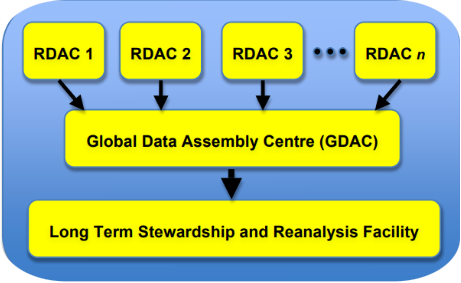
\includegraphics[width=0.75\textwidth]{../images/schematicTaskSharing.drawio.png}
    \caption{Schematic of the GHRSST Regional/Global Task Sharing (R/GTS) framework.}
    \label{fig:r/gts}
\end{figure}
\par\vspace{0.25cm}
Since large-scale GHRSST data production and dissemination commenced in 2006, the GHRSST GDAC and LTSRF have combined to provide over 50,000 users more than 100 terabytes of GHRSST data. Over 28 terabytes of data are in NODC\'s LTSRF holdings with another approximately 10 Terabyte added each year. The detailed interactions of the R/GTS components are described in the GHRSST Interface Control Document [AD-1].
Each component of the R/GTS is independently managed and operated by different institutions and agencies. The R/GTS itself is coordinated by the international GHRSST Science Team, which receives guidance and advice from the GHRSST Advisory Council. A GHRSST Project Office coordinates the overall framework. A full discussion of GHRSST over the last 10 years is reported in [RD-2] and [RD-3].
\subsection{Overview of the GDS 2.0}
The GHRSST R/GTS was made possible through the establishment of a rigorous GHRSST Technical Data Specification (GDS), which instructed international satellite data providers on how to process satellite data streams, defined the format and content of the data and metadata, and documented the basic approaches to providing uncertainty estimates and auxiliary data sets. The GHRSST-PP established the first GDS (v1.6) [RD-1], which formed the basis of all GHRSST data production from 2005 through 2011. In 2010 the Version 2 of the GDS described in this document will go into operations following a phased implementation schedule.
\par\vspace{0.25cm}
All GHRSST products entering the R/GTS must strictly follow the common GDS when generating L2P, L3, L4, and GMPE data. As a result, users with common tools to read data from one RDAC can securely use data from any of the others as well as the GDAC and LTSRF without a need to re-code. Table 6-1 provides a summary of GDS 2.0 data products and their basic characteristics.
\par\vspace{0.25cm}
The remainder of this document provides the detailed specifications for GHRSST L2P, L3, L4, and GMPE products, their file naming convention, metadata requirements, and all necessary tables, conventions, and best practices for creating and using GHRSST data.
\newp